\chapter*{Bilagor}
\addcontentsline{toc}{chapter}{Bilagor}
\appendix

\chapter{Rotationskurvor}\label{app-vrot}
\label{app:rotcurves}
En rotationskurva visar den cirkulära hastigheten som funktion av
radien. Inom astronomin använder man en galax rotationkurva för
att räkna ut dess massa. Här diskuterar vi tre exempel på
rotationskurvor och visar dem i figur~\ref{rotcurve}.

\section{Stelkroppsrörelse} 

Tänk dig en roterande stel kropp, tex en cd-skiva. Den roterar med
konstant vinkelhastighet $\Omega = \frac{V}{R} = {\rm
  konstant}$. Hastigheten är alltså proportionell mot radien:
\begin{equation}
V \propto R. 
\end{equation}


\section{Keplersk rotation: Solsystemet} 
\label{sect:kepler}

\begin{figure}[h]
\begin{center}
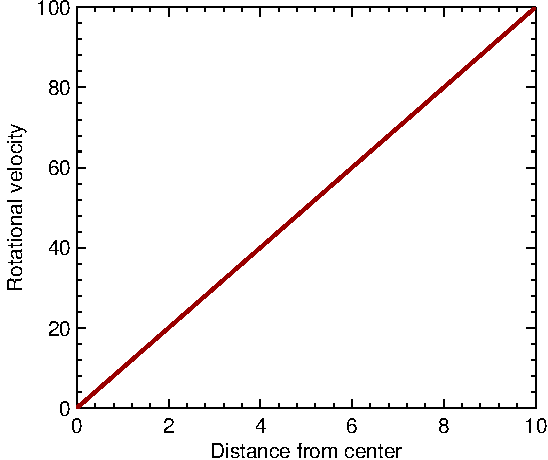
\includegraphics[width=8.2cm]{../figures/cdrot.pdf}
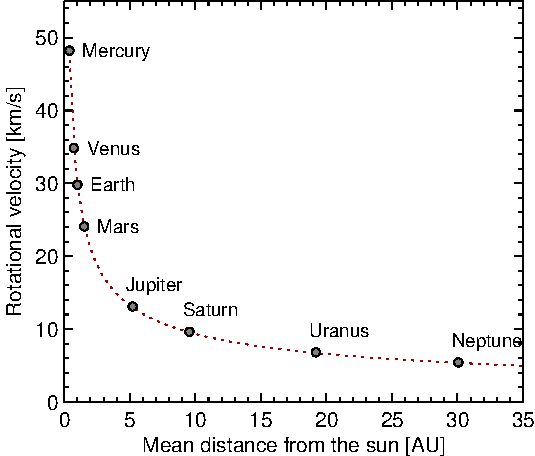
\includegraphics[width=8.2cm]{../figures/solsystrot.pdf}
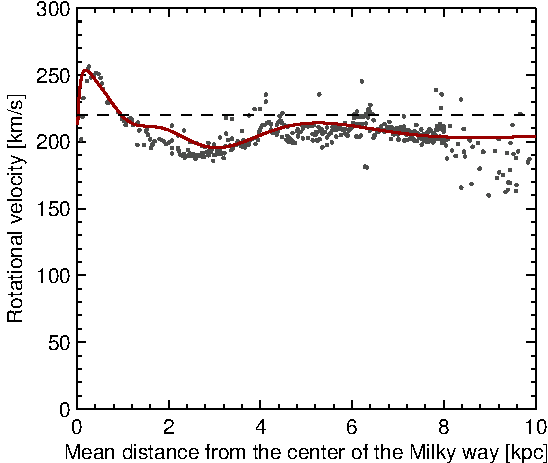
\includegraphics[width=8.2cm]{../figures/mwrot.pdf}
\end{center}
\caption{\emph{Uppe till vänster}: Stelkroppsrörelse (till exempel
  en roterande cd skiva) \emph{Uppe till höger}:
  Rotationshastigheterna för planeterna i solsystemet. Linjen
  motsvarar Keplers lag (ekvation.~(\ref{kepler})) med vilken
  planeters rörelse stämmer bra överens. Avståndsskalan är utritad i
  så kallade \emph{Astronomiska enheter} (AU) vilket är avståndet
  mellan jorden och solen. $1 \text{AU}=150\cdot 10^6
  \text{km}$. \emph{Nedre bilden}: Vintergatans rotationskurva
  (prickar) och en modell som beskriver mätningarna (linje). Eftersom
  materien i Vintergatan är utspridd över hela galaxen, följer inte
  rotationskurvan Keplers lag, som den skulle gjord om all materia var
  koncentrerad i mitten. (Data från Sofue et al, 2009) }
\label{rotcurve}
\end{figure}  

I solsystemet har planeterna en försumbar massa i jämförelse med
solens massa. Därför är masscentrum i solsystemet väldigt nära solens
centrum. Centrifugalaccelerationen från planeternas hastigheter
balanserar gravitationsaccelerationen:

\begin{equation}
\frac{V^2}{R}= \frac{GM}{R^2}
\end{equation}
där $M$ är massan och $G$ gravitationskonstanten. Man säger att
rotationskurvan är \emph{Keplersk} och hastigheterna minskar när
radien ökar.

\begin{equation}
\boxed{V_{\rm Keplerian}(R) = \sqrt{\frac{GM}{R}}.}
\label{kepler}
\end{equation}



\section{Rotationskurvan för en spiralgalax}

Rotationskurvorna för de flesta galaxer är konstanta efter en viss
radie ("platta") till skillnad från solsystemet där rotationskurvan
minskar med radien.

\begin{equation}
\boxed{V_{\rm Galaxy}(R) = {\rm constant}}
\end{equation}
Vinkelhastigheten,$\Omega$ , varierar med $\Omega \propto
1/R$. Materia nära centrum roterar med en högre vinkelhastighet,
jämfört med materia längre ut i en galax.

Vid stora radier är hastigheterna märkbart större än i det keplerska
fallet. Detta är en indikation på att det existerar extra materia
långt ut i galaxerna. Detta är ett indirekt sätt att visa att det
finns mörk materia i galaxer.


\chapter{21 cm observationer: En tillbakablick}\label{app-history}

Historien kring upptäckten av 21 cm linjen är fascinerande eftersom
den utspelar sig under andra världskriget då internationella
vetenskapskontakter var svåra och många forskare fick kämpa för att
upprätthålla sin forskning.

H.C. van de Hulst, en Holländsk student, presenterade en rapport vid
ett möte i Leiden 1944 där han visade att en hyperfin övergång för
neutralt väte producerar strålning med våglängden 21 cm. Van de Hulst
var precis som andra forskare vid den här tiden isolerade på grund av
nazisternas ockupation. En artikel publicerades 1945 i en Holländsk
tidskrift.

Efter kriget började flera forskargrupper i olika länder bygga
utrustning som kunde detektera 21 cm strålningen. Den observerades
först av Ewen \& Purcell den 21 mars 1951 i USA; och senare samma år i
Holland av Muller \& Oort i maj. Deras artiklar publicerades i samma
utgåva av tidskriften Nature samma år. 1952 upptäckte även
Christiansen och Hindman linjen i Australien.

Den första systematiska undersökningen av HI i vår Galax gjordes i
Holland av van de Hulst, Muller och Oort. De använde en parabol från
en tysk radarmottagare. Antennen var 7.5 m i diameter och
vinkelupplösningen var ungefär 2 grader.

\begin{figure}[h]
  \centering
  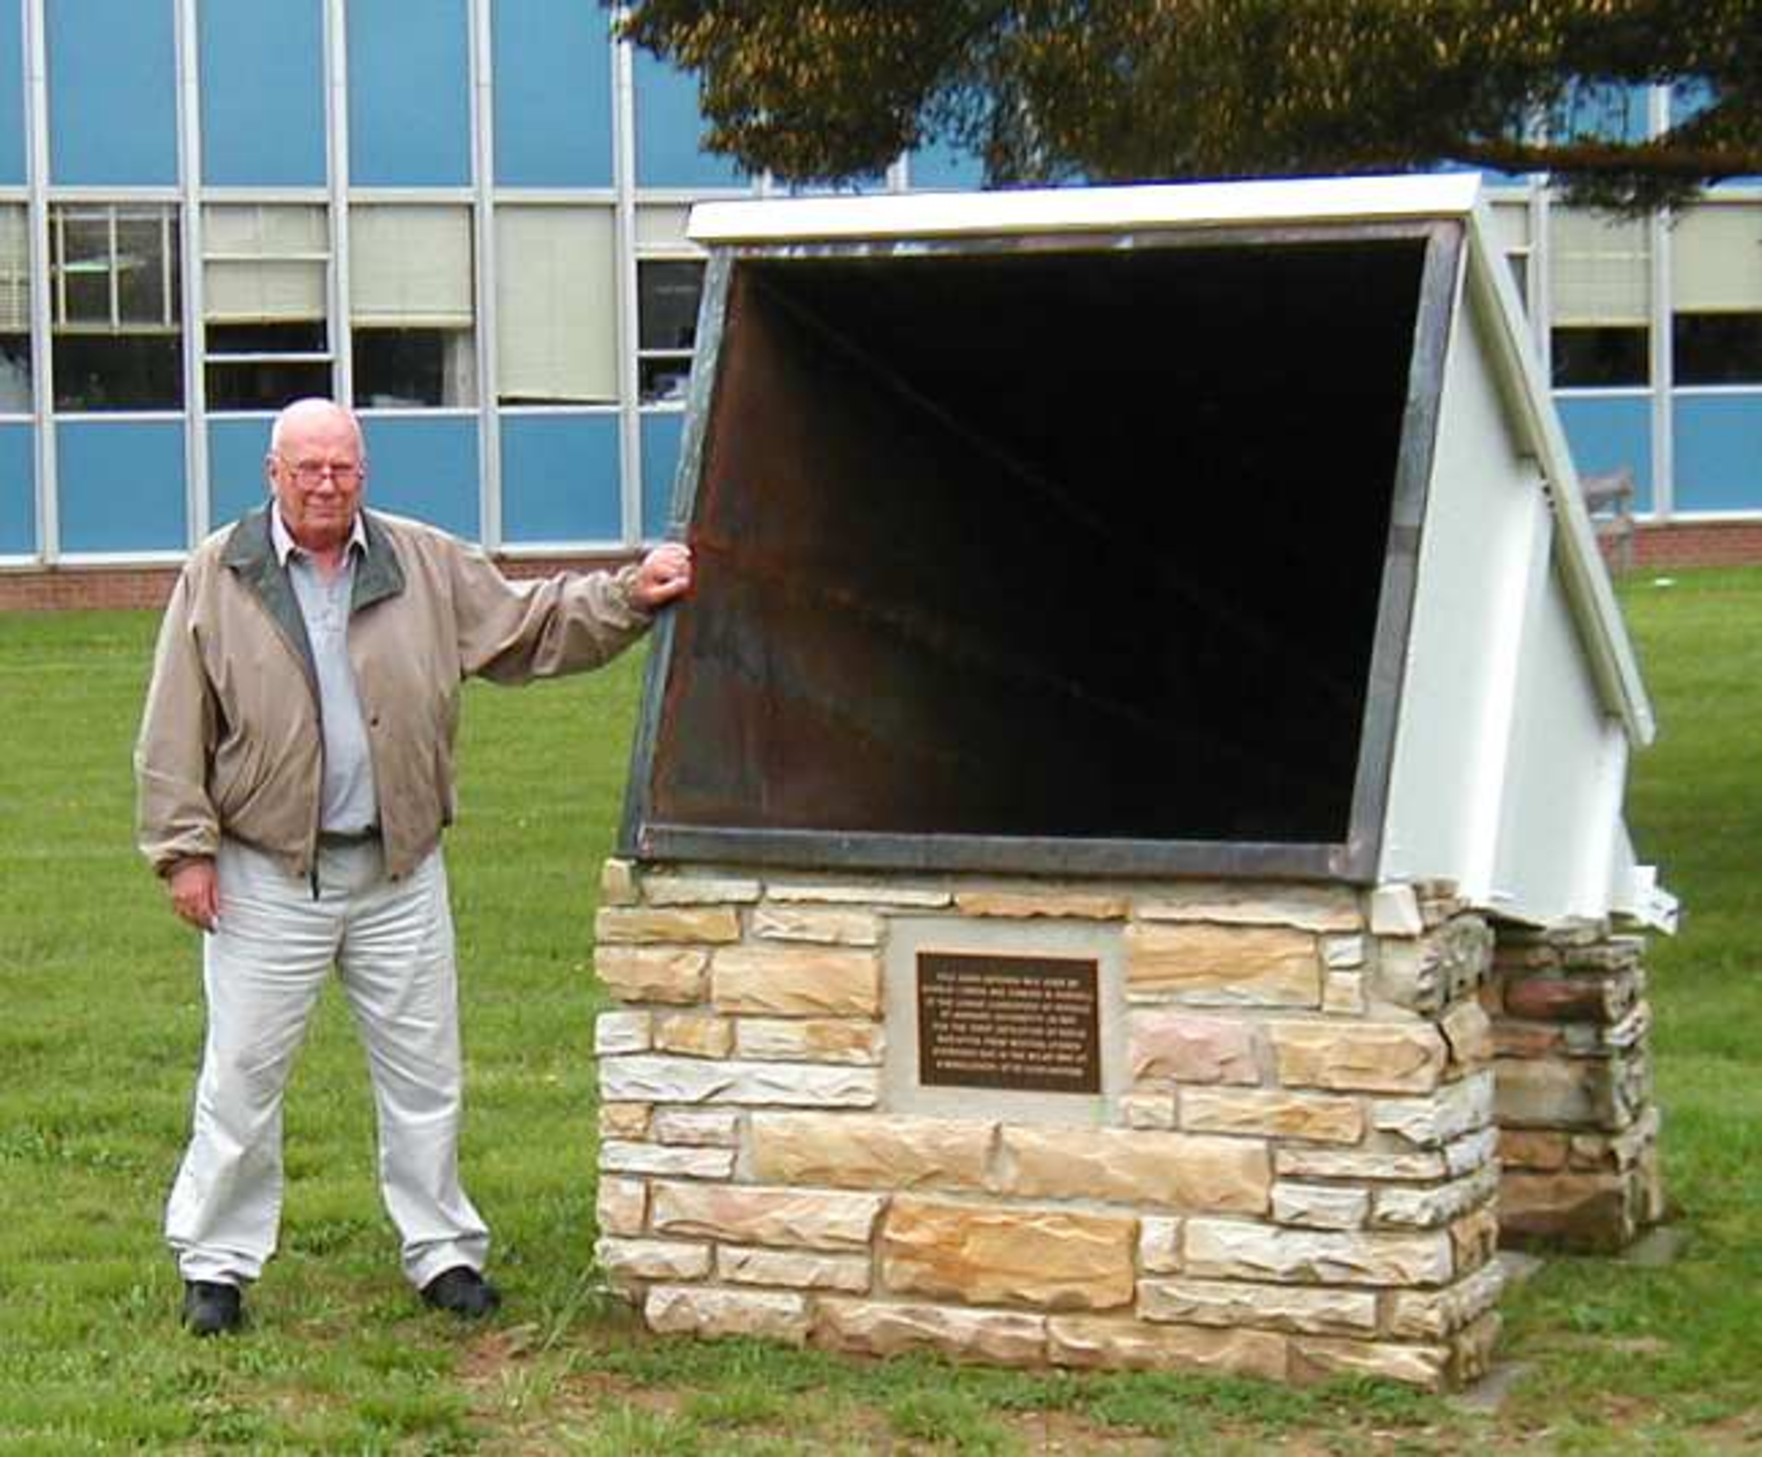
\includegraphics[width = 8 cm]{../figures/ev2.pdf}
  \caption{ H.I. (''Doc'') Ewen tillsammans med sin hornantenn vid ett
    besök till NRAO-Green Bank i Maj 2001. Han hade inte sett sin
    antenn sedan 1956!. (''NRAO / AUI / NSF'') }
  \label{fig:evpu}
\end{figure}
